\documentclass[twocolumn,a4paper]{article}

\usepackage{geometry}
\usepackage{hyperref}
\usepackage{enumitem}
\usepackage{tikz}
\usepackage{pgfplots}
\usepackage{amsmath}
\usepackage{colortbl}
\usepackage{mathpazo}
\usepackage{microtype}

\title{Exploring the Efficiency of Covering Locality-Sensitive Hashing}

\author{
  Kasper Kronborg Isager \\
  IT University of Copenhagen, Denmark \\
  \texttt{kasi@itu.dk}
  \and
  Radoslaw Niemczyk \\
  IT University of Copenhagen, Denmark \\
  \texttt{radn@itu.dk}
}

\date{\today}

\geometry{
  margin = 12mm,
  footskip = 6mm,
  columnsep = 9mm
}

\usetikzlibrary{
  matrix,
  positioning
}

\setlist{noitemsep}

\pgfplotsset{compat=1.9}

\newtheorem{definition}{Definition}
\newtheorem{example}{Example}

\begin{document}
  \maketitle

  \begin{abstract}
One of the latest developments in the area of locality-sensitive hashing (LSH) is the so-called \textit{covering LSH} scheme. This scheme solves one of the primary drawbacks of classic locality-senstive hashing, namely \textit{false negatives}, i.e. items that never collide with a query item despite them being similar. Covering LSH is therefore of interest in settings that require exact guarantees of producing a result, making classic LSH unsuitable as it only provides probabilistic guarantees. Given that the covering LSH scheme is still relatively new, it still lacks, to the best of our knowledge, a proper general-purpose implementation and associated evaluation thereof.

By implementing both the covering and the classic LSH schemes and benchmarking them on a real-world dataset designed for the evaluation of approximate nearest neighbour search algorithms, we show that within the same time and memory bounds, covering LSH is able to not only match but in fact outperform the filtering efficiency of classic LSH. This does however come at a negligible cost in insertion time and with an additional implementation specific memory overhead.
\end{abstract}

  \section{Introduction}
\label{introduction}

An increasingly popular approach for tackling similarity search in high-dimensional datasets is the so-called \textit{locality-sensitive hashing} (\textit{LSH}) technique, first presented by Piotr Indyk and Rajeev Motwani \cite{DBLP:conf/stoc/IndykM98}. LSH has therefore already found itself useful in a wide range of practical applications:

\begin{itemize}
  \item Nearest neighbour search
  \item Near-duplicate detection
  \item Hierarchical clustering
  \item Genome-wide association study
  \item Image and audio similarity identification
  \item Human fingerprint recognition
\end{itemize}

The basic idea of LSH is to hash items to buckets in a way that provides a higher probability of similar items being hashed to the same bucket than dissimilar items. Items that then hash to the same bucket despite them being dissimilar are \textit{false positives}. On the other hand, similar items that never hash to the same bucket are \textit{false negatives} \cite[p. 88]{DBLP:books/cu/LeskovecRU14}. While false positives have no effect on the precision of queries, false negatives may cause the algorithm to never consider items that are in fact the most similar to a query item. The latter becomes a problem in settings that require exact rather than probabilistic guarantees of returning a nearest neighbour, as is the case in for example human fingerprint recognition.

A recent paper by Rasmus Pagh \cite{DBLP:journals/corr/Pagh15} proposes an LSH scheme that completely does away with false negatives at a cost in efficiency. The purpose of our paper is to compare this LSH scheme, named \textit{covering LSH}, with classic LSH on a number of different metrics such as query throughput and filtering efficiency.

\paragraph{Organisation} This paper is organised as follows: In section \ref{background} we provide the background for classic LSH and outline the covering LSH scheme and the gurantees that it provides. In section \ref{implementation} we describe our implementation of the two LSH schemes. In section \ref{evaluation} an experimental evaluation based on a real dataset is made after which we compare the two LSH schemes. Finally, in section \ref{conclusion} we give our parting thoughts on the covering LSH scheme and the cost of the exact guarantees that it provides.

  \section{Background}
\label{background}

As touched upon in section \ref{introduction}, locality-sensitive hashing tackles the problem of similarity search in high-dimensional datasets by relaxing the requirement of finding exact nearest neighbours. Instead, LSH is used as an \textit{approximate} nearest neighbour algorithm, which inherently implies only probabilistic guarantees of finding a nearest neighbour. In general, LSH schemes act as randomized filters that attempt to reduce an input set to a subset of candidates for a given query item.

The formal definition of the approximate nearest neighbour problem for Hamming space is given as follows in \cite{DBLP:journals/corr/PhamP16}:

\begin{definition}
\label{definition-nearest-neighbour}
  Given a set $S \subset \{0, 1\}^d$, $|S| = n$, the Hamming distance function $D$, and parameters $r > 0$, $c > 1$, $\delta > 0$, construct a data structure such that, given any query $q \in \{0,1\}^d$, if there exists a point $x \in S$ and $D(x, q) \leq r$, it reports some point $y \in S$ where $D(y, q) \leq cr$ with probability $1 - \delta$.
\end{definition}

Here, $\delta$ defines the rate of occurences of false negatives.

The data structure mentioned in definition \ref{definition-nearest-neighbour} makes use of a family of \textit{locality-sensitive hash functions} in order to hash items to buckets. The definition of this family is given as follows in \cite{DBLP:conf/stoc/IndykM98}:

\begin{definition}
\label{definition-hash-functions}
  Given $r$, $c$, $p_1$, $p_2$, and $c > 1$, $p_1 < p_2$, a family $H = \{h \colon S \rightarrow U\}$ is said to be $(r, cr, p_1, p_2)$-sensitive for $(S, D)$ if for any $q,p \in S$ we have

  \begin{itemize}
    \item if $D(p, q) \leq r$ then $Pr_H [h(q) = h(p)] \geq p_1$,
    \item if $D(p, q) > cr$ then $Pr_H [h(q) = h(p)] \leq p_2$.
  \end{itemize}
\end{definition}

Here, $p_1$ is the lower bound on the probablity of close vectors colliding and $p_2$ is the upper bound on the probability of distant vectors colliding \cite[p. 100]{DBLP:books/cu/LeskovecRU14}. As such, we want $p_1$ to be close to 1 whereas we want $p_2$ to be close to 0. The intricate details of these collision probabilities will however not be touched more upon in this paper; we instead refer to \cite{DBLP:conf/stoc/IndykM98} and \cite{DBLP:books/cu/LeskovecRU14}.

\subsection{Classic LSH}
\label{background-classic-lsh}

The classic LSH scheme for Hamming space uses a random bit sampling approach for picking a number of components from an input vector. This sample is then used as the key in a map structure, which will be referred to as a \textit{partition}, for locating a bucket that the vector should be stored in. The bits to sample for a given partition are chosen independently and uniformly at random and stored with the partition. When looking for the nearest neighbour of a query vector, this sampling is repeated and the candidate vectors are those found in the bucket that the sample maps to.

\begin{example}
\label{example-classic-sampling}
Given input vector $v = 1101$, we randomly chose to sample component 1 and 3, giving us the key $v' = 10$. We then proceed to update our map structure with an entry for this key: $10 \rightarrow \{1101\}$

Given another input vector $u = 0110$, we again sample component 1 and 3, giving us the key $u' = 01$. We then add another entry to our map: $10 \rightarrow \{1101\}, 01 \rightarrow \{0110\}$.

Given a query vector $q = 1001$, we once again sample component 1 and 3, giving us the key $q' = 10$. We then look up this key in our map and receive the following set of candidates: $\{1101\}$.
\end{example}

\begin{figure}[ht]
  \centering
  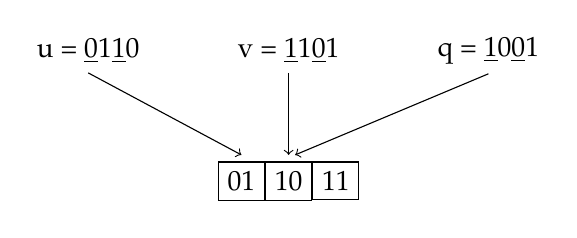
\begin{tikzpicture}
    \node (u) {u = \underline{0}1\underline{1}0};
    \node (v) [right=of u] {v = \underline{1}1\underline{0}1};
    \node (q) [right=of v] {q = \underline{1}0\underline{0}1};

    \matrix (m) [matrix of nodes, below=of v, row sep=-\pgflinewidth, style={nodes={draw}}]{
    01 & 10 & 11 \\
    };

    \path [->] (u.south) edge ([yshift=0.5ex] m-1-1.north);
    \path [->] (v.south) edge ([yshift=0.5ex] m-1-2.north);
    \path [->] (q.south) edge ([yshift=0.5ex, xshift=0.5ex] m-1-2.north);
  \end{tikzpicture}

  \caption{A graphical depiction of example \ref{example-classic-sampling}}
  \label{figure-classic-sampling}
\end{figure}

As can be seen in example \ref{example-classic-sampling}, $v$ and $u$ are not particularly similar as they only share a single component; by the sampling 1 and 3 they therefore do not map to the same bucket. However, $v$ and $q$ are almost identical as they share all but one component; the sampling 1 and 3 therefore maps them to the same bucket, albeit by chance. We have effectively reduced the set of potential candidates to half of the items in the original input set.

By adjusting the number of components sampled from vectors we can change the probability of collisions happening in the data structure. That is, by increasing the sample size we decrease the chance of vectors colliding, and vice versa, as more components would then have to match in order for a collision to happen.

If we want to keep the same sample size, but still increase the chance of vectors colliding, then we need to use more than one partition. Every partition will then indenpently chose the bits to sample and the set of candidate vectors will be the union of the vectors found in buckets in each partition.

\paragraph{Collision probabilities} By tweaking the sample size and the number of partitions to use, we can control the two probabilities $p_1$ and $p_2$ described in definition \ref{definition-hash-functions} \cite[p. 101]{DBLP:books/cu/LeskovecRU14}. By chosing a sample size $s$, the resulting probabilities will be $p_1' = p_1^s$ and  $p_2' = p_2^s$. On the other hand, by chosing a number of partitions 􏰄$b$, the resulting probabilities will be $p_1' = 1 - (1 - p_1)^b$ and $p_2' = 1 - (1 - p_2)^b􏰅$. By combining these, we get the probabilities $p_1' = 1 - (1 - p_1^s)^b$ and $p_2' = 1 - (1 - p_2^s)^b$. As such, both of these probabilities can be described by the equation $p = 1 - (1 - p^s)^b$, giving rise to what \cite[p. 89]{DBLP:books/cu/LeskovecRU14} calls the \textit{$S$-curve}:

\begin{figure}[ht]
  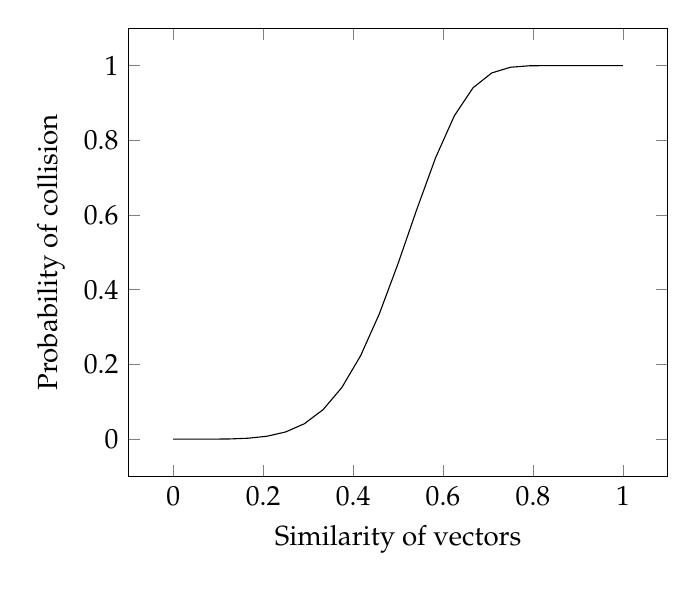
\begin{tikzpicture}
    \begin{axis}[xlabel = {Similarity of vectors}, ylabel = {Probability of collision}]
      \addplot[domain = 0:1]{1 - (1 - x^5)^20};
    \end{axis}
  \end{tikzpicture}

  \caption{The $S$-curve for $s = 5$, $b = 20$}
\end{figure}

\subsection{Covering LSH}
\label{background-covering-lsh}

\textit{To be written}

  \section{Implementation}
\label{implementation}

A library implementing both the classical and covering LSH schemes has been developed in order to facilitate an experimental evaluation of the two. The library has been released as open-source software and can be used freely\footnote{\url{https://github.com/kasperisager/hemingway}}.

  \section{Evaluation}
 \subsection{Data set}
 Our dataset is the set called \textit{ANN\_IFT1M}\footnote{\url{http://corpus-texmex.irisa.fr/}}. Which is a set of 1,000,000 vectors
 with dimensionality 128. Vectors are stored as raw little endians.
 This dataset is created especially for measurements of the approximate nearest 
neighbour searches.  
 \subsection{Metrics}
 \paragraph{Recall} Recall in information retrieval is the fraction of the data that are relevant to the query that are successfully retrieved.
 \paragraph{Precision} Precision is the fraction of retrieved data that are relevant to the query. Calculated by given formula:
 \paragraph{Time} We have three different speed metrics to compare:
 \begin{itemize}
  \item Construction time given in miliseconds. 
  \item Insertion time given in nanoseconds.
  \item Query time given in seconds.
\end{itemize}
 \paragraph{Memory consumptionl} Total amount of memory needed to create data structure and query it. Given in megabytes and gigabytes.
 \subsection{Benchmark} For measuring our metrics we are using library called 
 \textit{hayai}\footnote{\url{https://github.com/nickbruun/hayai}}, small C++ framework for writting benchmarks. It provides toolkit for measuring time, multiple runs and iterations.
  \subsection{Test environment} 
  Machine spec and software versions. 
\label{evaluation}

  \section{Conclusion}
\label{conclusion}

We have in this paper shown how the proposed covering LSH scheme performs compared to the classic LSH scheme when both are implemented as part of a general-purpose C++ library. Based on our evaluation, we can conclude that the query throughput of covering LSH outperforms that of classic LSH given the same time and memory bounds. This as a result of an improved distribution of items in buckets across partitions, which in turn reduces the average size of candidate sets for query items. The improved filtering efficiency does however come at a cost in the form of a decrease in insertion time and an additional memory overhead, both caused by the increased number of buckets.

In addition, our results verify the claim made in \cite{DBLP:journals/corr/Pagh15} that the efficiency of the covering LSH scheme matches that of the classic LSH scheme of \cite{DBLP:conf/stoc/IndykM98} in the case that $cr = \log n$. As stated earlier, the efficiency of our implementation in fact surpasses that of the classic LSH scheme while maintaining the exact guarantees of producing a nearest neighbour.


  \bibliographystyle{abbrv}
  \bibliography{tex/bibliography}
\end{document}
